\documentclass[11pt,a4paper]{article}
\usepackage{tikz}
\usetikzlibrary{arrows.meta,positioning}
\usepackage{tabularx}
\usepackage{amsmath,amssymb,amsthm}
\usepackage{geometry}
\geometry{margin=1in}
\usepackage{hyperref}
\usepackage{graphicx}
\usepackage{setspace}
\onehalfspacing

\title{\textbf{Paper B-02: Electrical Grids:\\ A Constraint-Driven Flux Dynamics (CDFD) Perspective}}
\author{Steve Bico Mujjabi, MD\\
\small Independent Researcher\\
\small Founder, Vura Labs\\
\small Kampala, Uganda\\
\small ORCID: 0009-0001-0556-5516}
\date{August 2026}

\begin{document}
\maketitle

% BEGIN SHARED-METHODS POINTER
\noindent\textit{Shared Part IV notation and evidence boundaries are defined in \path{PART_IV_METHODS_AND_CLAIM_BOUNDARY.md}. This paper states only its local observables, comparison, and failure conditions.}
% END SHARED-METHODS POINTER


\begin{abstract}
This paper develops a falsifiable CDFD/AFL model of Electrical Grids. It maps electrical demand, generation, and renewable variability to driving flux $\Phi$, thermal limits, stability margins, transmission, and reserve capacity to active constraint $C$, dispatch, storage, demand response, protection, and islanding to responsiveness $S$, and equipment aging, network state, prior contingencies, and operator learning to structural memory $M_s$. The target outcome is frequency stability, congestion, unserved energy, and restoration, tested against phasor measurements, dispatch records, topology, outage logs, and asset health. The paper treats universality as a shared model architecture rather than an assertion that unlike systems have the same material mechanism. It states the negative result that would make the mapping unnecessary and places the domain claim inside the cumulative CDFD programme and its reproducible runtime boundary.
\end{abstract}

\section{Introduction}

A power grid must perfectly balance electricity generation and consumption at every millisecond. When a transmission line trips due to a fault (e.g., a tree striking a wire), the current it was carrying instantly reroutes through adjacent lines. If those lines are already near their thermal capacity, they too will overheat and trip, triggering a chain reaction that can darken entire continents.

Engineers treat this as an operational reliability problem. CDFD treats it as a universal topological phenomenon. The grid is an active, constrained flow network attempting to maintain a critical mathematical equilibrium.

\section{The Grid as an Active Transport Surface}
We govern the electrical network using the Adaptive Operating Ratio:
\begin{equation}
    \Psi_s = \left( \frac{\Phi}{C} \right) \cdot S \cdot M_s
\end{equation}

For a node (substation) in the power grid:
\begin{itemize}
    \item \textbf{Flux ($\Phi$)}: The active power flow (Megawatts) passing through the node.
    \item \textbf{Constraint ($C$)}: The electrical impedance of the transmission lines and the hard thermal limits of the transformers.
    \item \textbf{Responsiveness ($S$)}: The grid's spinning reserve, battery capacitance, and the ability of automated relays to dynamically reroute power.
    \item \textbf{Memory ($M_s$)}: The physical, hardwired topology of the grid. Unlike the internet, which can dynamically rewrite software routes, power grid topology is highly rigid. This high memory locks the system's physical constraints into place.
\end{itemize}

\subsection{The Anatomy of a Cascading Blackout}
In standard operation, the grid remains near $\Psi_s \approx 1$. The generated flux $\Phi$ is comfortably handled by the constraints $C$.

When a major transmission line faults, its effective constraint $C$ instantly becomes infinite. The massive flux $\Phi$ it was carrying must redirect to a neighboring node. At this neighboring node, $\Phi$ spikes drastically. Because the physical wiring (the memory $M_s$) is rigid, the node's responsiveness $S$ cannot scale fast enough to accommodate the surge.

The node enters a severe over-flux regime ($\Psi_s \gg 1$). The intense flow physically damages the constraint structures (thermal melting of the line). To prevent total physical destruction, automated safety relays trip the line, effectively dropping $S \to 0$ and intentionally forcing the node into a dead state ($\Psi_s = 0$).

The flux $\Phi$ is then displaced again to the next neighbor, creating a moving wave of $\Psi_s \gg 1$ anomalies that systematically annihilate the network's active surface. This is a \textbf{Cascading Blackout}---the engineered equivalent of an ecological collapse.



\section{Measurement Layer}

% BEGIN PART IV MAJOR CROSS-DOMAIN UPGRADE
\section{Cross-Domain Model Upgrade: Mechanism, Scale, and Tests}

\subsection{Observable Translation}

The paper-specific translation begins with an observable chain rather than a
verbal analogy. For Electrical Grids, the proposed drive is electrical demand, generation, and renewable variability.
The active limitation is thermal limits, stability margins, transmission, and reserve capacity. Responsiveness is carried by
dispatch, storage, demand response, protection, and islanding, while retained state is represented by
equipment aging, network state, prior contingencies, and operator learning. The outcome to explain is frequency stability, congestion, unserved energy, and restoration.

\begin{table}[htbp]
\centering
\small
\caption{Operational CDFD/AFL map for Paper B-02.}
\begin{tabularx}{\textwidth}{|l|X|X|}
\hline
\textbf{Term} & \textbf{Paper-specific observable meaning} & \textbf{Measurement question} \\
\hline
$\Phi$ & electrical demand, generation, and renewable variability & What rate, load, gradient, or demand enters the focal system? \\
\hline
$C$ & thermal limits, stability margins, transmission, and reserve capacity & Which measured bottleneck limits transfer, function, or recovery? \\
\hline
$S$ & dispatch, storage, demand response, protection, and islanding & Which process changes effective capacity or reroutes the load? \\
\hline
$M_s$ & equipment aging, network state, prior contingencies, and operator learning & Which retained state makes equal present loads produce different futures? \\
\hline
$Y$ & frequency stability, congestion, unserved energy, and restoration & Which outcome is predicted out of sample, with uncertainty? \\
\hline
\end{tabularx}
\end{table}

\begin{figure}[htbp]
\centering
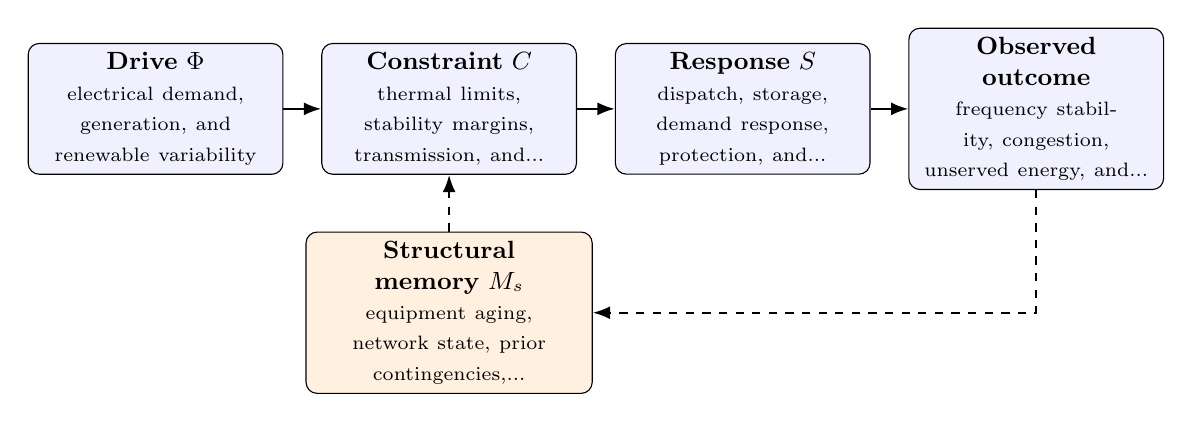
\begin{tikzpicture}[
    node distance=0.48cm,
    every node/.style={font=\small},
    box/.style={draw, rounded corners, align=center, minimum height=1.45cm, text width=3.0cm, fill=blue!6},
    memory/.style={draw, rounded corners, align=center, minimum height=1.25cm, text width=3.4cm, fill=orange!12},
    flow/.style={-{Latex[length=2.2mm]}, thick},
    feedback/.style={-{Latex[length=2.2mm]}, thick, dashed}
]
\node[box] (drive) {\textbf{Drive $\Phi$}\\\scriptsize electrical demand, generation, and renewable variability};
\node[box, right=of drive] (constraint) {\textbf{Constraint $C$}\\\scriptsize thermal limits, stability margins, transmission, and...};
\node[box, right=of constraint] (response) {\textbf{Response $S$}\\\scriptsize dispatch, storage, demand response, protection, and...};
\node[box, right=of response] (outcome) {\textbf{Observed outcome}\\\scriptsize frequency stability, congestion, unserved energy, and...};
\node[memory, below=0.72cm of constraint] (memory) {\textbf{Structural memory $M_s$}\\\scriptsize equipment aging, network state, prior contingencies,...};
\draw[flow] (drive) -- (constraint);
\draw[flow] (constraint) -- (response);
\draw[flow] (response) -- (outcome);
\draw[feedback] (outcome.south) |- (memory.east);
\draw[feedback] (memory.north) -- (constraint.south);
\end{tikzpicture}
\caption{Paper B-02 observable CDFD/AFL architecture for Electrical Grids. Solid arrows give the proposed forward chain; dashed arrows make history-dependent feedback explicit.}
\label{fig:b02-architecture}
\end{figure}

\subsection{Paper-Specific Causal Hypothesis}

For this paper, the hypothesized causal sequence is specific. A change in
electrical demand, generation, and renewable variability arrives faster than dispatch, storage, demand response, protection, and islanding can compensate.
This raises or redistributes thermal limits, stability margins, transmission, and reserve capacity. If the load persists,
the retained state encoded by equipment aging, network state, prior contingencies, and operator learning changes the next response, so a later event of equal
magnitude can produce a different trajectory in frequency stability, congestion, unserved energy, and restoration. The
scientific task is to estimate that sequence against the best ordinary model of
the domain, not merely to redescribe the outcome after it occurs.

\subsection{Cross-Scale Translation Without Mechanistic Erasure}

For the engineered systems family, the cross-domain translation compares demand, designed capacity, feedback control, dependency topology, and accumulated technical state. The strongest engineering use is prospective: the mapping must identify a bottleneck, a control action, or a recovery signature before the failure occurs. \cite{BarabasiAlbert1999,WattsStrogatz1998,Shannon1948,BakTangWiesenfeld1987}
The required scale declaration for this paper is milliseconds to decades; devices to interconnections. At short
scales, the key question is whether the incoming drive is transmitted,
buffered, or diverted. At intermediate scales, response changes effective
capacity and network exposure. At long scales, retained structure can alter the
state space itself. A result is genuinely cross-scale only when the aggregation
rule is stated and the same conclusion is not an artifact of averaging.

\subsection{Evidence Ladder and Discriminating Tests}

\begin{table}[htbp]
\centering
\small
\caption{Evidence ladder for Paper B-02. Each rung can fail independently.}
\begin{tabularx}{\textwidth}{|p{0.17\textwidth}|X|X|}
\hline
\textbf{Test} & \textbf{Design} & \textbf{Discriminating result} \\
\hline
Proxy audit & Measure phasor measurements, dispatch records, topology, outage logs, and asset health and preregister how each record maps to $\Phi$, $C$, $S$, $M_s$, and $Y$. & The mapping fails if proxies are non-identifiable, circular, or change meaning across cases. \\
\hline
Load ramp & Apply or observe a line or generator loss during high demand while estimating the dominant constraint and response time. & A threshold claim requires a reproducible nonlinear change and uncertainty bounds, not a visually chosen breakpoint. \\
\hline
Recovery and memory & Match present load across units with different histories, then compare recovery paths. & The memory claim requires history-dependent divergence after current conditions are controlled. \\
\hline
Model comparison & Compare the baseline domain model with and without the CDFD/AFL state variables using held-out data. & The paper's stated falsifier is: the mapping adds no value beyond established power-flow and stability models. \\
\hline
\end{tabularx}
\end{table}

\subsection{Research Programme and Boundary Conditions}

The immediate research programme has four steps. First, construct a documented
dataset from phasor measurements, dispatch records, topology, outage logs, and asset health and retain raw units before normalization.
Second, fit a baseline domain model and report its calibration and out-of-sample
error. Third, add the smallest identifiable CDFD/AFL state extension and test
whether it improves prediction of frequency stability, congestion, unserved energy, and restoration. Fourth, repeat the
analysis across the declared scale range and publish negative cases as part of
the cross-domain translation audit.

% END PART IV MAJOR CROSS-DOMAIN UPGRADE

\section{Conclusion}
Power grids are thermodynamic surfaces highly vulnerable to constraint-locking. By utilizing CDFD, grid operators can move beyond localized thermal monitoring and instead track the systemic $\Psi_s$ topology of the network in real-time, deliberately isolating high-flux bottlenecks before they trigger a catastrophic macroscopic phase shift.
\section*{Conflict of Interest} The author declares no conflict of interest.
\section*{Data Availability}
Part-specific runtime diagnostics are under each Part's \path{outputs/} directory.

Release-wide code: \path{Part_E_Synthesis/supplementary/}.

Generated summaries: \path{Part_E_Synthesis/outputs/}.

Figures: \path{Part_E_Synthesis/figures/}.


\section{Reference Layer}
\bibliographystyle{plain}
\bibliography{universal_afl_references}
\end{document}
